% Solution: Tadelis (2013) Exercise 8.8 "Entry Deterrence 1". Input by \solitem.
% Reused from lista-reais-lectures-01-04-solutions/item13.tex, deepened (mixed Nash equilibria,
% value of commitment, link to the Brexit lessons). Check: check_B_L04.py.
\begin{exsol}{Tadelis Exercise 8.8}{171--172}{Foundations}{2}
\asked Set up the game tree of the entry story (NSG enters or not, then S\&P fights or
accommodates) and find the subgame-perfect equilibrium outcome.

\method Backward induction in a finite game of perfect information (Lecture~3, slide~30; Tadelis
\S8.1, Def.~8.1 and Prop.~8.1, pp.~152--153). With perfect information the subgame-perfect
equilibria are exactly the profiles that survive backward induction (Lecture~4, slide~17; Tadelis
\S8.2, p.~157). Non-credible threats in Nash equilibrium: Lecture~4, slides~8 and~13. Same structure
as the entry game of Cabral \S7.2 (\texttt{Notas/L03/L03-06}).

\solution
\textbf{Notation.} Players: NSG (the entrant, E) and S\&P (the incumbent, I). E chooses
$\mathit{In}$ or $\mathit{Out}$; after $\mathit{In}$, I chooses $W$ (price war) or $A$
(accommodate). Payoffs $(u_E, u_I)$ in \$ million of net present value. The entry cost of 2 is
sunk once E enters, so it is subtracted from every payoff that follows $\mathit{In}$:
\begin{align*}
  (u_E,u_I)(\mathit{Out}) &= (0,\ 10),\\
  (u_E,u_I)(\mathit{In},W) &= (1-2,\ 1) = (-1,\ 1),\\
  (u_E,u_I)(\mathit{In},A) &= (4-2,\ 4) = (2,\ 4).
\end{align*}
\begin{center}
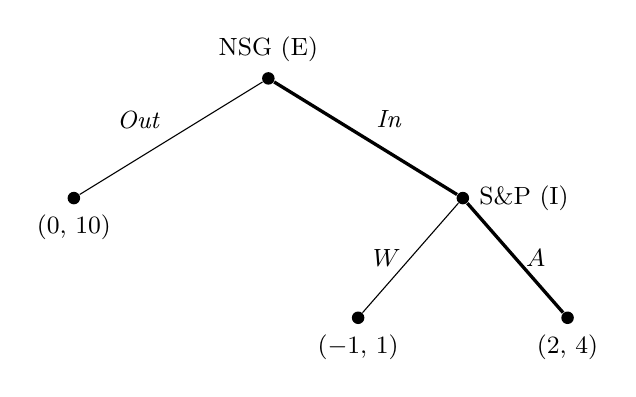
\begin{tikzpicture}[scale=0.95,dot/.style={circle,fill,inner sep=1.6pt},
  every node/.style={font=\small}]
  \node[dot,label=above:{NSG (E)}] (r) at (0,0) {};
  \node[dot,label=below:{$(0,\,10)$}] (o) at (-2.6,-1.6) {};
  \node[dot,label=right:{S\&P (I)}] (i) at (2.6,-1.6) {};
  \node[dot,label=below:{$(-1,\,1)$}] (w) at (1.2,-3.2) {};
  \node[dot,label=below:{$(2,\,4)$}] (a) at (4.0,-3.2) {};
  \draw (r) -- node[above left] {$\mathit{Out}$} (o);
  \draw[very thick] (r) -- node[above right] {$\mathit{In}$} (i);
  \draw (i) -- node[left] {$W$} (w);
  \draw[very thick] (i) -- node[right] {$A$} (a);
\end{tikzpicture}\\[2pt]
{\footnotesize Payoffs $(u_E, u_I)$; thick branches = backward-induction choices.}
\end{center}

\textbf{Step 1: the incumbent's node.} After entry, S\&P compares
\[
  u_I(\mathit{In},A) = 4 > 1 = u_I(\mathit{In},W),
\]
so it accommodates. The price war is not a credible response.

\textbf{Step 2: the entrant's node.} Replacing S\&P's node by its outcome $(2,4)$, NSG compares
\[
  u_E(\mathit{In}) = 2 > 0 = u_E(\mathit{Out}),
\]
so it enters. SPE: $(\mathit{In}, A)$, outcome entry and accommodation, payoffs $(2,4)$. The game
has two proper subgames (the whole game and the one at S\&P's node), and the SPE plays a Nash
equilibrium in both.

\textbf{Step 3: all Nash equilibria.} Normal form (rows: E's strategies; columns: I's strategies):
\begin{center}
\begin{tabular}{r|c|c|}
\multicolumn{1}{r}{} & \multicolumn{1}{c}{$W$} & \multicolumn{1}{c}{$A$}\\ \cline{2-3}
$\mathit{Out}$ & $\br{0},\ \br{10}$ & $0,\ \br{10}$ \\ \cline{2-3}
$\mathit{In}$ & $-1,\ 1$ & $\br{2},\ \br{4}$ \\ \cline{2-3}
\end{tabular}
\end{center}
Pure Nash equilibria: $(\mathit{In},A)$ and $(\mathit{Out},W)$. With $w = \Pr_I(W)$, NSG's
payoff from entering is $-w + 2(1-w) = 2 - 3w$, so $\mathit{Out}$ is a best reply iff
$0 \ge 2 - 3w$, i.e.\ $w \ge \frac23$; S\&P is not reached and is indifferent. The full set is
\[
  \{(\mathit{In}, A)\} \ \cup\ \{(\mathit{Out},\ w\,W + (1-w)A) : w \ge \tfrac23\}.
\]
Every equilibrium in the second family fails sequential rationality at the node S\&P never reaches
(Tadelis Def.~8.1, p.~152): the threat ``war with probability at least $\frac23$'' costs nothing
because it is never carried out, and it would not be carried out ($1 < 4$).

\textbf{Step 4: what would make the threat credible (deepening).} Suppose S\&P could, before NSG
decides, commit to a penalty $b$ that it pays if it accommodates (a public contract, a capacity
investment, a ``most-favored-customer'' clause). Then at its node S\&P fights iff $1 > 4 - b$,
i.e.\ $b > 3$; NSG, anticipating war, stays out ($-1 < 0$), and S\&P earns 10 without ever paying
$b$. A credible commitment is worth up to $10 - 4 = 6$ to S\&P. Independently, an entry cost above 4
would deter entry even with accommodation ($4 - \text{cost} < 0$).

\interp S\&P's prediction of a price war is cheap talk: once NSG has sunk its \$2 million, a war
gives S\&P 1 instead of 4, and NSG knows it. These are the three lessons of the Brexit case
(Lecture~4, slide~11) in miniature: \emph{talk is cheap} (announcing war without changing payoffs is
not credible); \emph{sunk investments can be strategic} (only a sunk, payoff-changing move such as
the penalty $b$ makes war credible); \emph{observability matters} (the commitment works only if NSG
sees it before deciding). The outcome does not depend on how the entry cost is booked: if ``each
firm earns \$1 million'' were already net of it, NSG would still enter ($2 > 0$, and even a war
would pay $1 > 0$).

\verify \texttt{check\_B\_L04.py} recomputes both backward-induction steps, the two pure Nash
equilibria of the $2\times2$ normal form, scans $w$ on a grid of step $\frac1{300}$ (Nash equilibria
exactly at $w = 0$ with entry and $w \ge \frac23$ with $\mathit{Out}$), and checks the commitment
thresholds $b > 3$ and the value $6$. Output line: \texttt{tadelis-8-8: SPE (In, A); NE (Out, Pr(W)
>= 2/3); commitment worth up to 6}. Tadelis prints no answer.

\mistakes
\begin{itemize}
  \item Forgetting to subtract the sunk entry cost from NSG's payoffs after entry.
  \item Reporting $(\mathit{Out}, W)$ as an SPE because it is a Nash equilibrium.
  \item Giving the outcome only (``NSG enters'') when the SPE is a strategy profile: S\&P's plan
  $A$ must be stated.
\end{itemize}

\answer{Tree above. Subgame-perfect equilibrium: NSG plays $\mathit{In}$, S\&P plays $A$
(accommodate); outcome: entry and accommodation, payoffs $(2, 4)$ in \$ million (NSG net of the
entry cost). The other Nash equilibria, $\mathit{Out}$ with $\Pr(W) \ge \frac23$, rest on a
non-credible threat.}
\end{exsol}
